\chapter{$VH (H \rightarrow b\bar{b}/c\bar{c})$ Combined Analysis}\label{chap-VH}
\ChapFrame

\textit{Perhaps the most important \textit{raison d'être} of the \textit{Large Hadron Collider} (LHC) was to discover the Brout-Englert-Higgs boson (Higgs - $H$), a feat achieved by the ATLAS and CMS Experiments in July 2012 \cite{ATLAS:2012yve, CMS:2012qbp}. Theorised in 1964 by two independent papers introducing the mechanism of spontaneous symmetry breaking to give mass to the gauge bosons \cite{Englert:1964et,  PhysRevLett.13.508}, its discovery almost fifty years later marked one of the greatest achievements of the particle physics community. The Higgs boson is an essential part of the \glsfirst{sm} as it is tied to the mechanism through which particles acquire mass without breaking the electroweak gauge invariance, as described in Chapter \ref{chap-theory}. While the gauge bosons $W$ and $Z$ gain mass through symmetry breaking, in the \gls{sm} the fermions - quarks and leptons - acquire theirs by interacting with the Higgs fields -  a scalar field carried by the Higgs boson $H$, as described by the Yukawa mechanism \cite{10.1143/PTPS.1.1}.}\\

\section{Introduction}
The Higgs boson $H$ \cite{Englert:1964et, PhysRevLett.13.508, Higgs:1964ia, PhysRevLett.13.585} was discovered in 2012 by the ATlAS and CMS Collaborations using their Run 1 data of the \gls{lhc} \cite{ATLAS:2012yve, CMS:2012qbp}. This triggered a race by both experiments to study the specific properties of the discovered particle, and in particular to observe its different production processes and decay channels. The initial decay channels studied for the groundbreaking discovery where the bosonic decays of the Higgs to final states of photons and leptons: $H \rightarrow \gamma\gamma$, $H \rightarrow ZZ$, and $H \rightarrow WW$. These channels benefit from clean experiment conditions, reliable measurements, and limited backgrounds. The new particle has been studied in ever finer detail, confirming its coupling to many massive particles of the \gls{sm} and showing remarkable agreement with the properties dictated by the theory. During the \gls{lhc} Run 2, corresponding to data taken from 2015 to 2018, the $t\bar{t}H$ production mechanism was observed for the first time, providing the first measurement of the top Yukawa coupling \cite{ATLAS:2018mme, CMS:2018uxb}. Additionally, the decay of Higgs bosons to a pair of $\tau$-lepton is now well established and different cross-sections measurements have been performed \cite{atlasTauMeasu, CMS:2021gxc}. Importantly, the decay channel of the Higgs boson to a $b\bar{b}$ pair was observed by both ATLAS and CMS \cite{ATLAS:2018kot, CMS:2018nsn}. This last decay channel is of particular significance since it has the largest predicted branching ratio of 58\% for $m_H = 125$ GeV in the \gls{sm}, providing the first evidence of the decay of the Higgs to second-generation fermions. \\ 

Concerning the second generation of fermions, there now is evidence of the decay to a $\mu^-\mu^+$ pair by CMS \cite{CMS:2020xwi} and a 2$\sigma$ excess over the background-only hypethesis by ATLAS \cite{ATLAS:2020fzp}. Furthermore, constraints on the branching ratio of the $H$ to another second-generation fermion, the $c$-quark, have been set by both collaborations studying the $H \rightarrow c\bar{c}$ decay mode \cite{Aaboud:2018fhh}. This decay mode is the most common Higgs decay mode that has yet to be observed. It is indeed particularly challenging due to the small predicted branching ratio of 2.9\% \cite{DJOUADI199856}, the large background rates, and the experimental difficulties in identifying $c$-jets. It is a fertile ground for new physics \glsfirst{bsm} due to the smallness of the predicted Yukawa coupling $y^{\textrm{SM}}_c \approx 3.99 \times 10^{-3} $ \cite{yukawac} for the $c$-quark as well as an important test of the validity of the model \cite{PhysRevD.89.033014, PhysRevD.92.033016, Botella:2016krk, PhysRevD.98.055001, GHOSH2016504, PhysRevLett.123.031802, PhysRevD.100.115041}. The fermion Yukawa couplings in the \gls{sm} were indeed added ad-hoc and there is a distinct mass hierarchy between the three generations of quarks that can be probed by studying their coupling strengths to the Higgs boson. In the $VH (H \rightarrow b\bar{b}/c\bar{c})$ analysis, to which this chapter is dedicated, the hierarchy of mass between the $b$- and $c$-quark, respectively a $3^{\textrm{rd}}$ and $2^{\textrm{nd}}$ generation quark, is probed.

\section{The $VH (H \rightarrow b\bar{b})$ and $VH (H \rightarrow c\bar{c})$ ATLAS Analyses}
While $H \rightarrow b\bar{b}$ enjoys the largest branching ratio at the observed Higgs mass, the large multi-jet background in a hadron collider like the \gls{lhc} makes this decay mode very challenging. The measurements for both the $b\bar{b}$ and $c\bar{c}$ decay modes are therefore performed in a so-called \textit{associated production mode}, where the $H$ is produced in addition to an extra vector boson $V$ ($W$ or $Z$) decaying leptonically, to electrons ($e$), muons ($\mu$), neutrinos ($\nu$), or a combination $e\nu$ or $\mu\nu$. Taus ($\tau$) are not currently included , in particular, to migrate 0L-channel events with a hadronically decaying $\tau$ to the 1L channel. Despite the relatively small cross-section of the $VH$ production mode ($\sigma_{VH}$ = 2.25 pb compared to the total $H$ production $\sigma_H \approx$ 51 pb), the process benefits from experimentally favourable conditions thanks to the presence of leptons in the event signature: these allow for efficient triggering and greatly reduce the contribution of the multi-jet background. Other analyses relying on full-hadronic final states in the associated or other production modes are also performed in ATLAS but are less sensitive to the Higgs coupling to heavy-flavour quarks. In the ATLAS Collaboration, the $VH (H\rightarrow b\bar{b})$ and $VH (H\rightarrow c\bar{c})$ analyses adopt very similar strategies. The main ingredient is the ability to reliably tag the flavour of jets produced in an event to reconstruct the heavy quark pair produced in the $H$ decay, using the tools described in Chapter \ref{chap-ftag}. \\ % sentence on taus strange

Using the full Run 2 dataset with a total integrated luminosity of 140 fb$^{-1}$, the published $VH (H\rightarrow c\bar{c})$ ATLAS analysis obtained the following upper limits on the signal strength of the $VH (H\rightarrow c\bar{c})$ as predicted by the \gls{sm}: an observed (expected) upper limit of 26 $\times$ \gls{sm} (31 $\times$ \gls{sm}) \cite{Collaboration:2721696}. The measurement also provided the first constraint on the Higgs-charm coupling modified $|\kappa_c| < 8.5$. For comparison, CMS reported an observed (expected) upper limit of 14.4 $\times$ \gls{sm} (7.6 $\times$ \gls{sm}) and a constraint of $1.1 < \kappa_c < 5.5$ \cite{arXiv:2205.05550}. \\  % quote stxs

For the $VH (H\rightarrow b\bar{b})$, thanks to a larger expected signal, the analysis reaches a sensitivity of 6.7 standard deviations \cite{ATLAS:2020fcp}. Following observation, the focus of this analysis has shifted towards a precision differential measurement of the fiducial cross-sections as a function of momentum in the reduced \glsfirst{stxs} scheme. To probe larger $p_T$ ranges, the analysis is now split into the \textit{resolved} \cite{ATLAS:2020fcp} and the \textit{boosted} \cite{ATLAS:2020jwz} analyses, with the latter restricting to values of the transverse momentum of the associated vector boson $p_T^V$ above 250 GeV. The name of these analyses comes from the ability to independently resolve the two $b$-jets from the Higgs decay into two distinct small cone radius (small-$R$) jets at low $p_T^V$. At high $p_T^V$, the Higgs $p_T^H$ is highly Lorentz-boosted requiring a change of strategy: the candidate Higgs are efficiently reconstructed as a single large-radius ($R = 1$) jet merging the two $b$-jets. The measured signal strengths, the ratio of the measured yield to the \gls{sm} predictions, are: 
\begin{itemize}
\item For the resolved analysis in Run 2: a signal strength of $1.02_{-0.17}^{+0.18}$ corresponding to an observed (expected) significance of 6.7 (6.7) standard deviations \cite{ATLAS:2020fcp}. Due to the good sensitivity of the analysis, the result is further detailed into the $WH$ and $ZH$ production processes with observed (expected) significances of, respectively, 4.0 (4.1) and 5.3 (5.1) standard deviations. Furthermore, the $VH$ cross-section times the $H \rightarrow b\bar{b}$ and $V\rightarrow$ leptons branchings fractions ($\sigma \times BR$) are reported in the reduced \gls{stxs} scheme. Finally, limits are set on the coefficients of effective Lagrangian operators which can affect the $VH$ production and the $H \rightarrow b\bar{b}$ decay.
\item For the boosted analysis: a signal strength of  $0.72_{-0.36}^{+0.39}$ corresponding to an observed (expected) significance of 2.1 (2.7) standard deviations \cite{ATLAS:2020jwz}.
\end{itemize}

Some preliminary studies aiming at combining the different analyses have already been performed, with the resolved $VH (H\rightarrow b\bar{b})$ and $VH (H\rightarrow c\bar{c})$ analyses combined in Ref \cite{Collaboration:2721696} and the resolved and boosted $VH (H \rightarrow b\bar{b})$ combined\footnote{CMS published an analoguous combined analysis in Ref \cite{CMS-PAS-HIG-20-001}.} in Ref \cite{ATLAS:2021wqh}. These required careful studies to remove the overlap between the analyses, such as by introduceing a switch in $p_T^V$ at 400 GeV between the resolved and boosted strategies. However, these first combinations used the published analyses and the objective of the new Combined Analysis is to define a common analysis strategy, correlating as much as possible the experimental and modelling uncertainties for both Higgs decay modes and $p_T^H$ regimes, thereby improving the measurements of $VH (H \rightarrow b\bar{b})$ and $VH (H \rightarrow c\bar{c})$ simultaneously. This new combined measurement has several additional benefits: 
\begin{itemize}
\item The Higgs-charm and -beauty coupling modifiers $\kappa_c$ and $\kappa_b$ can be measured directly, as well as their ratio $\kappa_c/\kappa_b$. 
\item The auxiliary measurements of background processes are shared, leading to a better knowledge of background processes that contribute to both phase spaces such as the $V$+jets and top-quark processes.
\item The combined analysis benefits from improved signal selection thanks to upgraded physics objects and event reconstruction techniques. In particular, new machine learning-based techniques are integrated for both the event selection and flavour tagging.
\end{itemize}

The rest of this chapter focuses on the current state of the $VH (H\rightarrow b\bar{b}/c\bar{c})$ Combined Analysis, as the analysis is not yet concluded. The stage described corresponds to that attained at the end of the first three unblinding approval reviews. Some modifications to the analysis can be expected in the soon-to-be-published result, in particular to the fit framework and main deliverables. The work presented here is largely based on the internal analysis notes of the experimental team and personal work carried out during the duration of the DPhil project. 

\section{Overview of the Combined $VH (H\rightarrow b\bar{b}/c\bar{c})$ Analysis}
The Combined Analysis is performed with the full ATLAS Run 2 proton-proton collision data, collected from 2015 to 2018, for a total integrated luminosity of 140 fb$^{-1}$ at a centre of mass energy $\sqrt{s} = 13$ TeV. The regions and boundaries between the different regimes of the analysis are illustrated in Figure~\ref{fig:ana-strat}. The $VH (H\rightarrow b\bar{b})$ and $VH (H\rightarrow c\bar{c})$ analyses are separated by the required presence of two $b$-tagged jets or a $c$-tagged jets respectively. The $p_T^V$ cut marks the difference between the Higgs candidate reconstruction scheme of the resolved and boosted $VH (H\rightarrow b\bar{b})$: two small radius (R = 0.4) jets below a $p_T^V$ of 400 GeV and above one large radius (R = 1) jets with two $b$-tagged sub-jets made by \glsfirst{vr} track jet associated to the large-$R$ jet.

\begin{figure}[h!]
\center
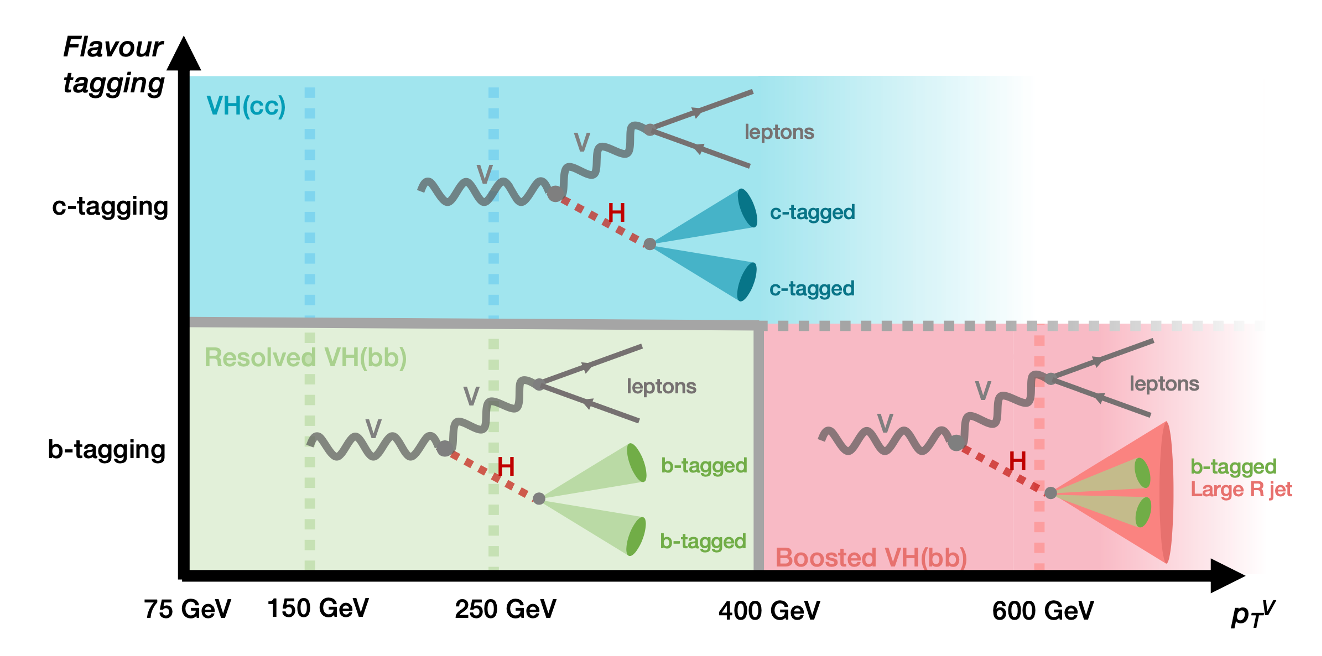
\includegraphics[width=\textwidth]{Images/VH/Cat/AnalysisRegime.png}
\caption{The analysis regimes considered in the combined $VH (H\rightarrow b\bar{b}/c\bar{c})$ analysis, from the internal documentation.} 
\label{fig:ana-strat}
\end{figure}

For each analysis region, three channels are defined based on the decay mode of the vector boson $V$: $Z \rightarrow \nu \nu$ defines the \textit{0-lepton} (0L), $W \rightarrow \ell \nu $ the \textit{1-lepton} (1L), and $Z \rightarrow\ell^+\ell^-$ the \textit{2-lepton} (2L), where $l$ refers to an electron or a muon and $\nu$ to a neutrino. The signal considered are the  $VH (H\rightarrow b\bar{b})$ and $VH (H\rightarrow c\bar{c})$ processes, with the \gls{sm} diboson processes $VZ (Z\rightarrow b\bar{b})$ and $VZ (Z\rightarrow c\bar{c})$ considered as signals in a cross-check analysis. Having a larger cross-section and being kinematically similar to the signals, these processes can be measured with good statistical significance, thereby offering a suitable test case to verify the performance of the strategy deployed. The main backgrounds are the production of a vector boson with additional jets($V$+jets, mostly $Z$+jets in 0L and 2L, $W$+jets in 1L) and the top-quark processes (\textit{Top}, predominantly the top-quark pair production $t\bar{t}$, with one of the $t$ decaying leptonically, and a sub-leading contribution from single top-quark production with an extra $W$ boson, both in 0L and 1L). Minor backgrounds are the \gls{qcd} multi-jet\footnote{Thanks to the required presence of leptons in the final state.}, the single top process (without an extra associated $W$ boson) and non-signal diboson pair productions ($VV$). \\ 

Flavour tagging plays an essential role in the analysis, splitting the analysis phase space into different regimes of studies. The most important backgrounds are also split based on flavour components. The $V+$jets is split into three components: $V+$ heavy flavour jets ($V+$hf, including $V+bb$ and $V+cc$), $V+$ mixed flavour ($V+$mf, including the $V+bc$, $V+bl$, and $V+cl$), and the $V+$ light jet ($V+l$, including all other possible flavour selection including $\tau$'s). The top-quark background is also split by flavour: the Top(bb), in which the two selected jets are $b$-tagged, is treated separately from the Top(bbbq) which groups all other flavours as it is the dominant flavour background in $VH(H\rightarrow b\bar{b})$. \\

All backgrounds are simulated using \glsfirst{mc} simulation packages, except for the multi-jet which is estimated from a data-driven method\footnote{The top background in 2L is also estimated using data-driven techniques.} in the 1L channel and is negligible in other channels. To reproduce the conditions of the ATLAS detector, simulated samples are passed through the GEANT4 software \cite{Agostinelli:602040} and the ATLAS reconstruction software. The chapter is separated into different section introducing the datasets and simulation (Section \ref{sec-datasets}), a description of the reconstructed object (Section \ref{sec-obj}), the analysis selection and regimes (Section \ref{sec-regimeCat}), the event categorisation (Section \ref{sec-eventCat}), the modelling (Section \ref{sec-modelling}), the fit framework (Section \ref{sec-fitFramework}), and finally the main results (Section \ref{}).
% TODO adapt the outline for the final one.

\section{Data and Simulated Samples}\label{sec-datasets} % TODO check the lumi is not 139
The combined analysis is performed on data collected during the Run 2 of the \gls{lhc}, with proton-proton collisions recorded between 2015 and 2018 at a $\sqrt{s} = 13$ TeV for an integrated luminosity of 140 fb$^{-1}$ \cite{ATLAS:2022hro}. Data events must pass some quality requirements, ensuring for example that all the sub-detectors operated as expected. The analysis also requires accurate \glsfirst{mc}-based modelling of the signal and the background processes, except for the \gls{qcd} multi-jet and the \ttb background in the 2-lepton channel which have data-driven estimations. All \gls{mc} samples are simulated with the ATLAS detector effect \cite{ATLASSimulationInfra} using \textsc{Geant4} \cite{Agostinelli:602040}. The nominal samples are produced using the prescriptions described in Table \ref{tab:VHgenerators}, detailing the \gls{me} generators, parton showers and \glsfirst{pdf} releases used as well as the cross-sections. Samples are normalised either to the best theoretical cross-section predictions or the generator cross-sections. \\

\begin{table}
    \centering
    %\rotatebox{90}{
    \resizebox{\textwidth}{!}{
    \begin{tabular}{ l| l | l | l | l | l}
        \hline \hline
    Process & Matrix Element & PDF Set (ME) & Parton Shower & $\sigma$ order & $\sigma \times$ Br [pb] \\
     \hline \hline
     $qq \to WH \to \ell \nu b\bar{b}$ & PowHeg-Box v2 + GoSam + MiNLO & NNPDF3.0NLO & Pythia-8.245 & NNLO(QCD)+
    NLO(EW) & $2.69 \times 10^{-1}$ \\
     $qq \to ZH \to \nu \nu b\bar{b}$ & PowHeg-Box v2 + GoSam + MiNLO & NNPDF3.0NLO & Pythia-8.245 & NNLO(QCD)+
    NLO(EW) & $8.91 \times 10^{-2}$ \\
     $qq \to ZH \to \ell \ell b\bar{b}$ & PowHeg-Box v2 + GoSam + MiNLO & NNPDF3.0NLO & Pythia-8.245 & NNLO (QCD)+NLO(EW) & $4.48 \times 10^{-2}$ \\
     $gg \to ZH \to \nu \nu b\bar{b}$ & PowHeg-Box v2                   & NNPDF3.0NLO & Pythia-8.307 & NLO+NLL & $1.43 \times 10^{-2}$ \\
     $gg \to ZH \to \ell \ell b\bar{b}$ & PowHeg-Box v2                 & NNPDF3.0NLO & Pythia-8.307 & NLO+NLL & $7.23 \times 10^{-3}$ \\
     \hline
     $qq \to WH \to \ell \nu c\bar{c}$ & PowHeg-Box v2 + GoSam + MiNLO & NNPDF3.0NLO & Pythia-8.245 & NNLO(QCD)+
    NLO(EW) & $1.34 \times 10^{-2}$ \\
     $qq \to ZH \to \nu \nu c\bar{c}$ & PowHeg-Box v2 + GoSam + MiNLO & NNPDF3.0NLO & Pythia-8.245 & NNLO(QCD)+
    NLO(EW) & $4.42 \times 10^{-3}$ \\
     $qq \to ZH \to \ell \ell c\bar{c}$ & PowHeg-Box v2 + GoSam + MiNLO & NNPDF3.0NLO & Pythia-8.245 & NNLO (QCD)+NLO(EW) & $2.23 \times 10^{-3}$ \\
     $gg \to ZH \to \nu \nu c\bar{c}$ & PowHeg-Box v2                   & NNPDF3.0NLO & Pythia-8.307 & NLO+NLL & $7.10 \times 10^{-4}$ \\
     $gg \to ZH \to \ell \ell c\bar{c}$ & PowHeg-Box v2                 & NNPDF3.0NLO & Pythia-8.307 & NLO+NLL & $3.59 \times 10^{-4}$ \\
    % \hline
    %  $Z \to \nu \nu$ + jets   & Sherpa 2.2.1 & NNPDF3.0NNLO & Sherpa 2.2.1 & NNLO & 10700 \\
    %  $W \to \ell \nu$ + jets  & Sherpa 2.2.1 & NNPDF3.0NNLO & Sherpa 2.2.1 & NNLO & 60200 \\
    %  $Z \to \ell \ell$ + jets & Sherpa 2.2.1 & NNPDF3.0NNLO & Sherpa 2.2.1 & NNLO & 6300 \\
      \hline
      $W \to \ell \nu$ + jets  & Sherpa 2.2.11 & NNPDF3.0NNLO & Sherpa 2.2.11 & NNLO & 60242  \\
      $Z \to \ell \ell$ + jets & Sherpa 2.2.11 & NNPDF3.0NNLO & Sherpa 2.2.11 & NNLO & 6201   \\
      $Z \to \nu \nu$ + jets   & Sherpa 2.2.11 & NNPDF3.0NNLO & Sherpa 2.2.11 & NNLO & 416.05  \\
      \hline
      \ttb   & Powheg-Box v2 & NNPDF3.0NLO & Pythia-8.230 & NNLO+NNLL &  704  \\
      single-top ($Wt$)  & Powheg-Box v2 & NNPDF3.0NLO & Pythia-8.230 & Approx. NNLO & 80.03  \\
      single-top ($t$)   & Powheg-Box v2 & NNPDF3.0NLO & Pythia-8.230 & NLO       & 70.7  \\
      single-top ($s$)   & Powheg-Box v2 & NNPDF3.0NLO & Pythia-8.230 & NLO       & 3.35  \\
    %  \hline
    %  $qq \to WW$ & Sherpa 2.2.1 & NNPDF3.0NNLO & Sherpa 2.2.1 & NLO & 45.7 \\
    %  $qq \to WZ$ & Sherpa 2.2.1 & NNPDF3.0NNLO & Sherpa 2.2.1 & NLO & 21.7 \\
    %  $qq \to ZZ$ & Sherpa 2.2.1 & NNPDF3.0NNLO & Sherpa 2.2.1 & NLO & 6.53 \\
      \hline
      $qq \to WW$ & Sherpa 2.2.11 & NNPDF3.0NNLO & Sherpa 2.2.11 & NLO & 47.93 \\
      $qq \to WZ$ & Sherpa 2.2.11 & NNPDF3.0NNLO & Sherpa 2.2.11 & NLO & 20.85 \\
      $qq \to ZZ$ & Sherpa 2.2.11 & NNPDF3.0NNLO & Sherpa 2.2.11 & NLO & 6.33 \\
      $gg \to VV$ & Sherpa 2.2.2 & NNPDF3.0NNLO  & Sherpa 2.2.2 & NLO & 2.78 \\
     \hline \hline
    \end{tabular}
    }
    \caption{The nominal Monte Carlo samples used in the \vhbc\ analysis, and the corresponding process cross-sections at $\sqrt{s} = 13$ TeV. The PDF sets in the table are the ones used for the matrix element.}
    \label{tab:VHgenerators}
\end{table}
    

Both simulated samples and data are reconstructed with the offline reconstruction software of ATLAS. The \textsc{EvtGen} 1.6.0 program is used to simulate the properties of $b$- and $c$-hadrons decays\footnote{\textsc{EvtGen} 1.7.0 is used for the \textsc{Sherpa} generated samples.} \cite{LANGE2001152}. Pile-up is also included in the simulation, both from multiple interactions in the same and adjacent bunch crossing. This is performed by overlaying events with minimum bias simulated using \textsc{\textsc{Pythia}} 8 with A3 tune and interfaced with the \textsc{NNPDF} 2.3 \gls{pdf}s \cite{SJOSTRAND2015159}. The rest of this section gives more details behind the simulation of the different processes. When relevant, alternative samples generated from a different setup to the nominal samples are introduced. These alternative samples are used to assess modelling uncertainties.

\subsection{Signal Processes}
The analysis targets the \vhb\ and \vhc\ processes, here called \textit{signals}. The leading order (LO) Feynman diagrams contributing to the associated production $VH$ are the $qq$-initiated modes depicted in Figure~\ref{fig:feynloVH}. A gluon-initiated production of $ZH$ is also possible at next-to-leading order (NLO) with a quark loop (mostly top-quark), as depicted in Figure~\ref{fig:feynnloVH}. The \gls{me} calculations are based on the \textsc{Powheg-Box v2} generator \cite{StefanoFrixione_20072, POWHEGBOX}. The $qq$-initiated $VH$ samples have a \textsc{Powheg} generator with the multiscale improved NLO (MiNLO) procedure \cite{powhegHW}, with one-loop amplitudes computed with the GoSam automated software \cite{gosam}. The $qq$-initiated samples simulate \gls{ps}, \gls{ue}, and multiple parton interactions with \textsc{Pythia} 8.245, while the $gg$-initiated use \textsc{Pythia} 8.307 \cite{SJOSTRAND2015159}. Both use the AZNLO tune \cite{measureZGboson} with \gls{pdf}s based on the \textsc{NNPDF3.0NLO} for matrix elements \cite{PDFLHCrun2}. \\

\begin{figure}[h!]
  \center
  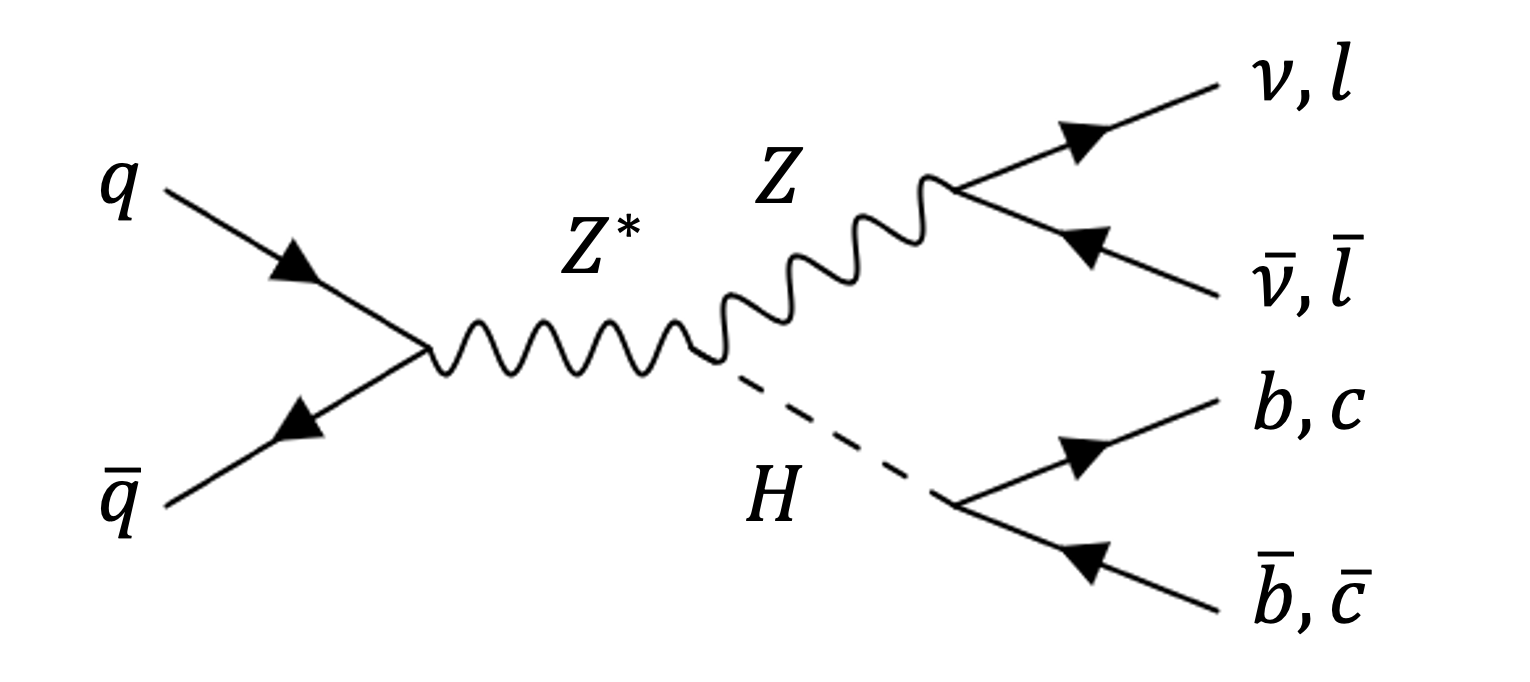
\includegraphics[width=0.48\textwidth]{Images/VH/Feynman/zh.png}
  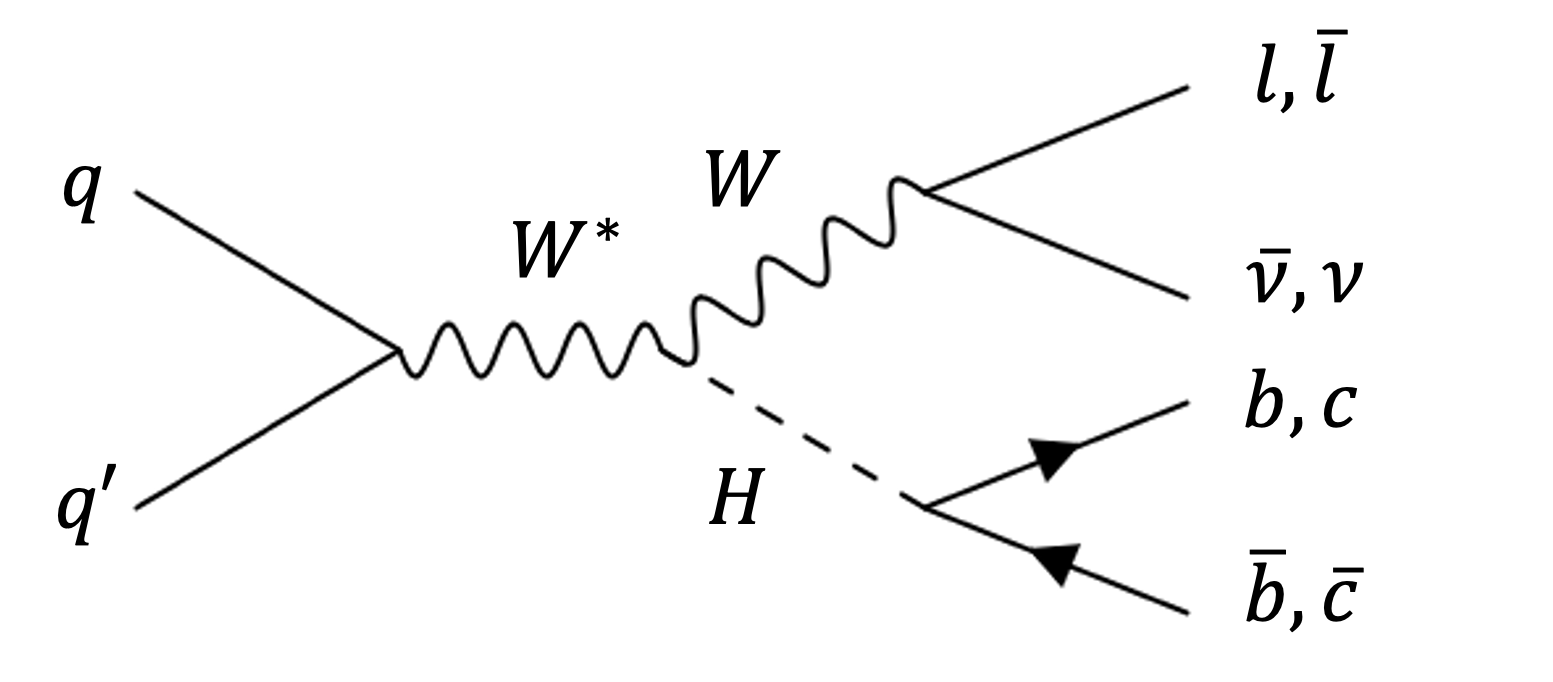
\includegraphics[width=0.48\textwidth]{Images/VH/Feynman/wh.png}
  \caption{Leading order Feynman diagrams for \vhbc, $qq$-initiated with $V$ decaying into leptons.} 
  \label{fig:feynloVH}
\end{figure}

\begin{figure}[h!]
  \center
  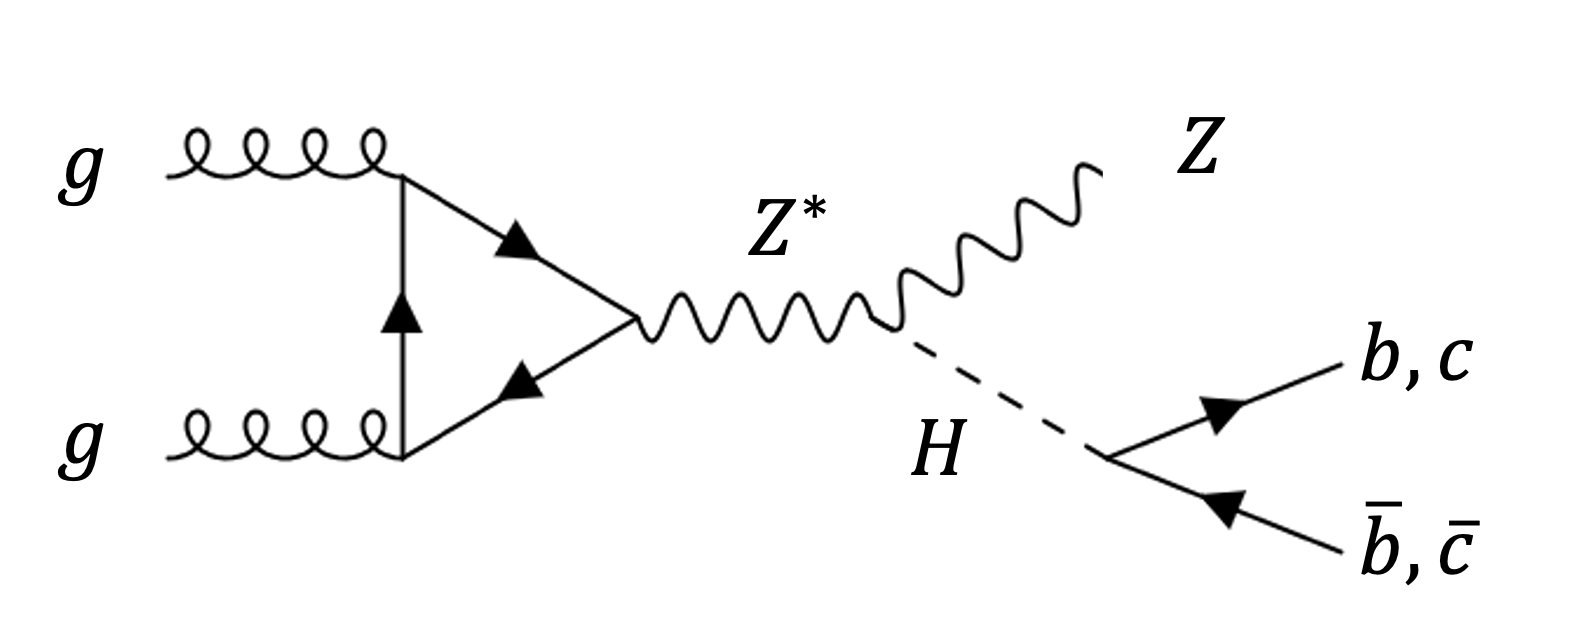
\includegraphics[width=0.48\textwidth]{Images/VH/Feynman/vh2order.png}
  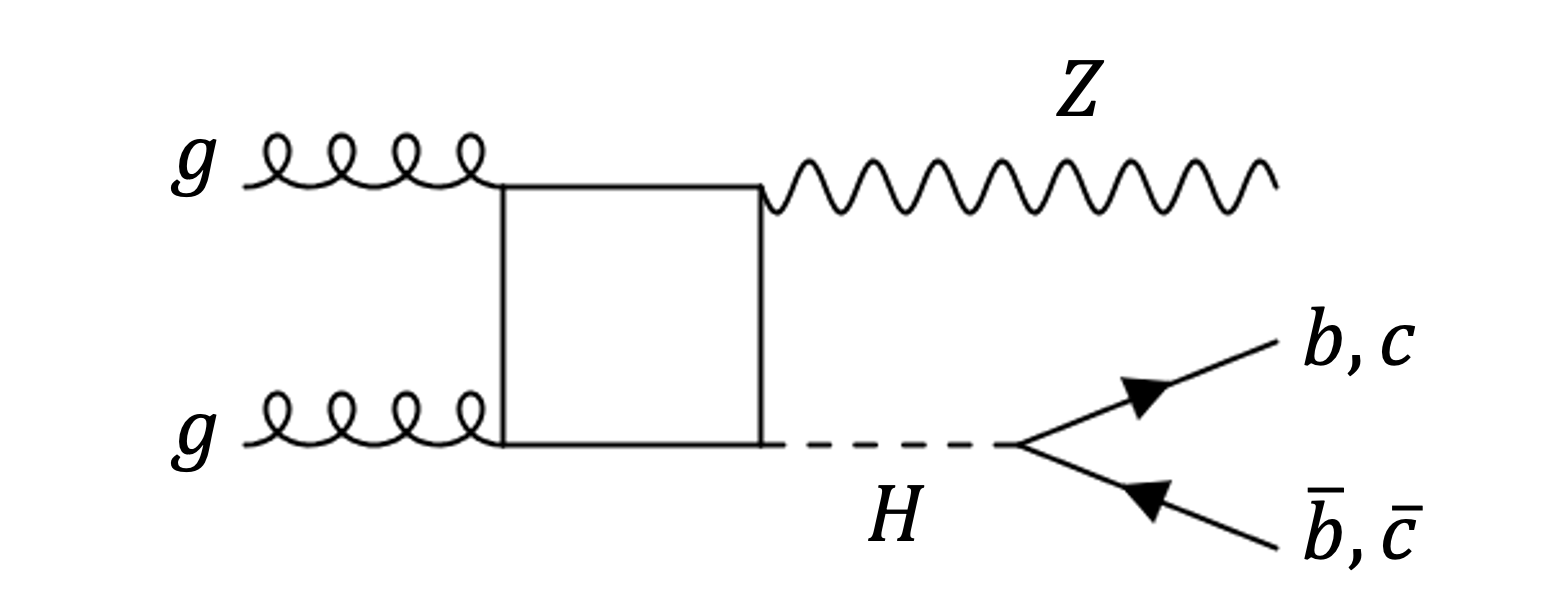
\includegraphics[width=0.48\textwidth]{Images/VH/Feynman/vh3order.png}
  \caption{Feynman diagrams of the $gg$-initiated contributions to $ZH(H\rightarrow b\bar{b}/c\bar{c})$.} 
  \label{fig:feynnloVH}
\end{figure}

The inclusive cross-sections for $WH$ and $ZH$ are calculated at NNLO in \gls{qcd} \cite{BREIN2004149} and NLO in electroweak \cite{PDFLHCrun2}. The $gg$-initiaed $ZH$ contribution relies on the LO prediction from \textsc{Powheg} instantiated with \textsc{Pythia} 8.

\paragraph{Alternative samples:} are simulated with \textsc{Powheg}+MiNLO+\textsc{Herwig} 7.0, with the same simulation stack as the nominal but replacing \textsc{Pythia} 8 by \textsc{Herwig} 7.0 \cite{bellm2017herwig} for the simulation of the \gls{ps}, hadrnonisation, \gls{ue}, and multiple parton interactions.

\subsection{Background Processes}
The most important backgrounds in the analyses are simulated with \gls{mc}, except for the multi-jet and the top backgrounds in the 2-lepton channel. These processes and their simulations are detailed in this section.

\subsubsection{$V+$jets}
The production of a gauge vector boson $V$ in association with jets is the largest background in the analysis. Some of the leading contributing Feynman diagrams to this process that can be selected are presented in Figure~\ref{fig:feynVJ}. Both the $Z+$jets and $W+$jets are simulated with \textsc{Sherpa} 2.2.11 \cite{10.21468/SciPostPhys.7.3.034}, which deliver NLO precision on matrix element computation for up to 2 jets and LO accuracy for between 3 and 5 jets. \gls{ps} and hadronisation are treated by the default \textsc{Sherpa} generator, with the NNLO \gls{pdf}s based on NNPDF3.0nnlo \cite{PDFLHCrun2}. Uncertainties from missing higher orders are evaluated by varying the \gls{qcd} renormalisation ($\mu_r$) and factorisation ($\mu_f$) scales in the matrix elements by respective factors 0.5 and 2. Flavour filtering is applied to generate samples with selected heavy flavour quarks.

\begin{figure}[h!]
  \center
  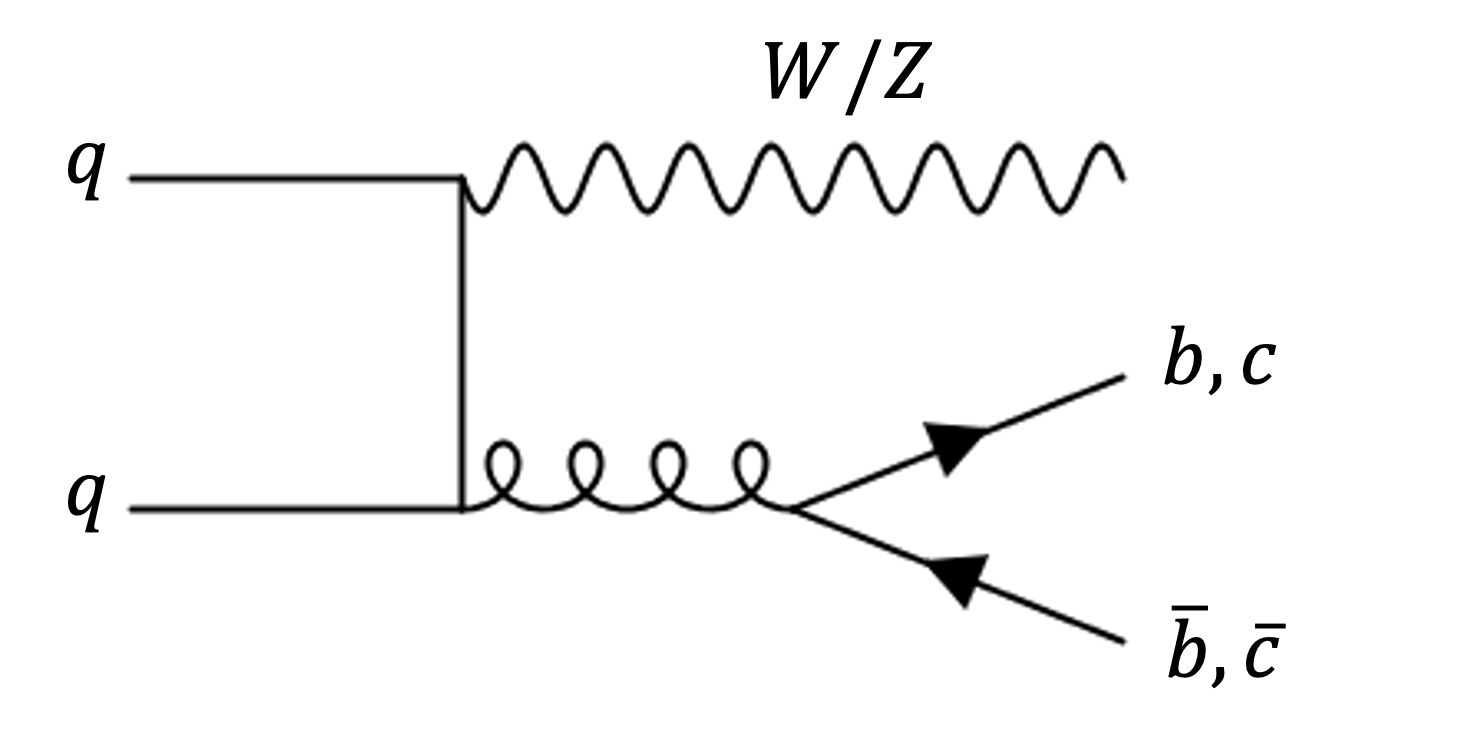
\includegraphics[width=0.48\textwidth]{Images/VH/Feynman/vjet.png}
  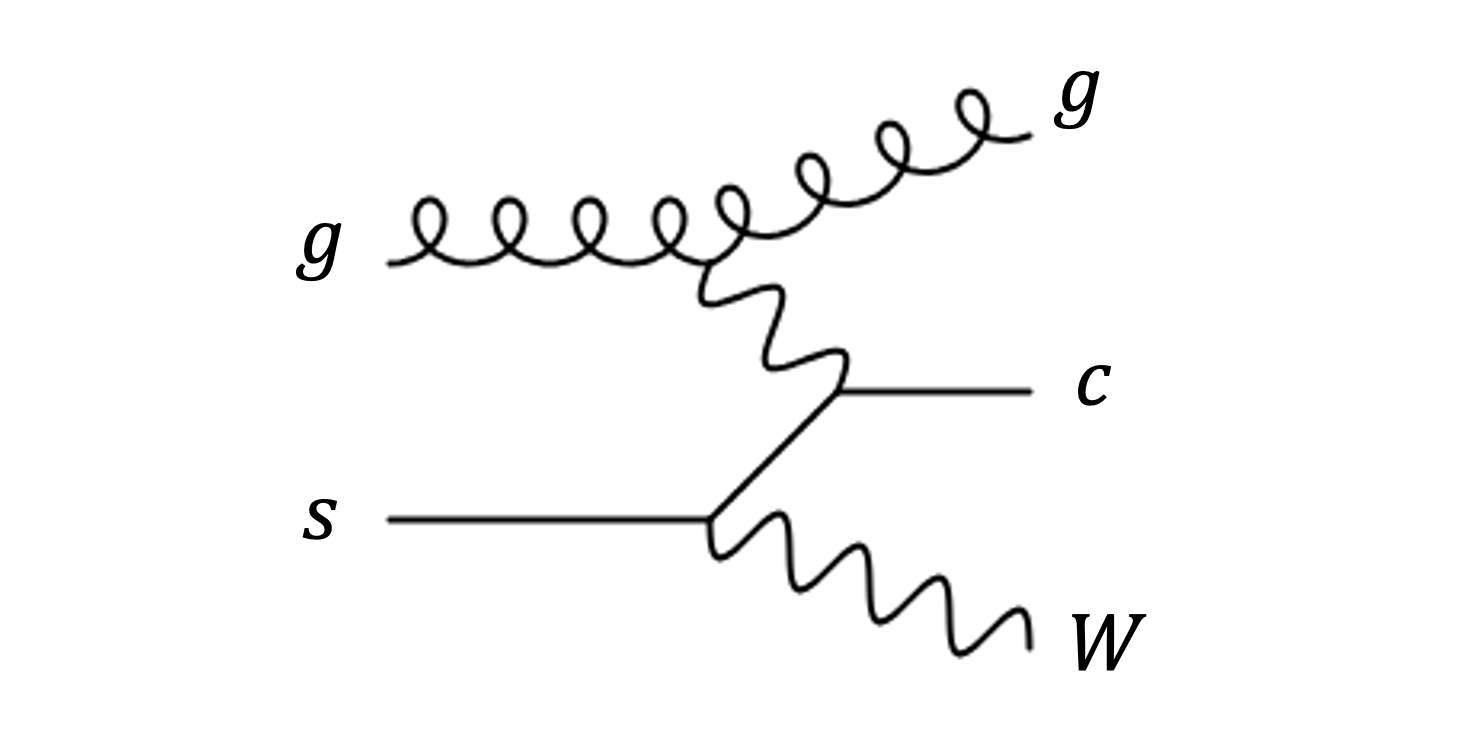
\includegraphics[width=0.48\textwidth]{Images/VH/Feynman/vjet2.png}
  \caption{Examples of Feynman diagrams of the $V+$jets process. The left diagram gives a same flavour jet pair due to the gluon splitting, while the right one can give mixed flavours.} 
  \label{fig:feynVJ}
\end{figure}

\paragraph{Alternative samples} Two sets of alternative samples are available:
\begin{itemize}
  \item \textsc{MadGraph FxFx} samples are produced for the modelling studies, using the \textsc{MadGraph5\_aMC\@NLO} 2.6.5 program \cite{madgraph}. This generates the $V$ boson with up to three additional partons in the final state at NLO accuracy. The scales $\mu_r$ and $\mu_f$ are set to 1/2 the transverse mass of all final-state partons + leptons. \textsc{Pythia} 8.240 is interfaced for showering and hadronisation, with the A14 tune and the NNPDF2.3lo \gls{pdf} set with $\alpha_s = 0.13$.
  \item \textsc{Sherpa} 2.2.1 \cite{sherpa2.2paper} samples are used as alternative generator as it gives different \ptv distributions to 2.2.11 \cite{simVjet}. These samples are similar to those used in the standalone \vhc \cite{Collaboration:2721696}.
\end{itemize}

\subsubsection{Top-pair Production}
The \ttb process is the second most important background in the analysis. The leading order Feynman diagram for this process is shown in Figure \ref{fig:feynttb}. The nominal samples are generated for the 0L and 1L channels with \textsc{Powheg} at NLO calculation of the matrix element \cite{StefanoFrixione_2007, PaoloNason_2004}. It is interfaced with \textsc{Pythia} 8.230 with the NNPDF3.0NLO \gls{pdf}s using the A14 tune for \gls{ps}, hadronisation, and \gls{ue} description. Filtering is applied while simulating to enhance statistics. Cross-sections are calculated to NNLO in \gls{qcd}, with resummation of the next-to-next-to-leading logarithmic (NNLL) soft gluon terms \cite{CZAKON20142930}.

\begin{figure}[h!]
  \center
  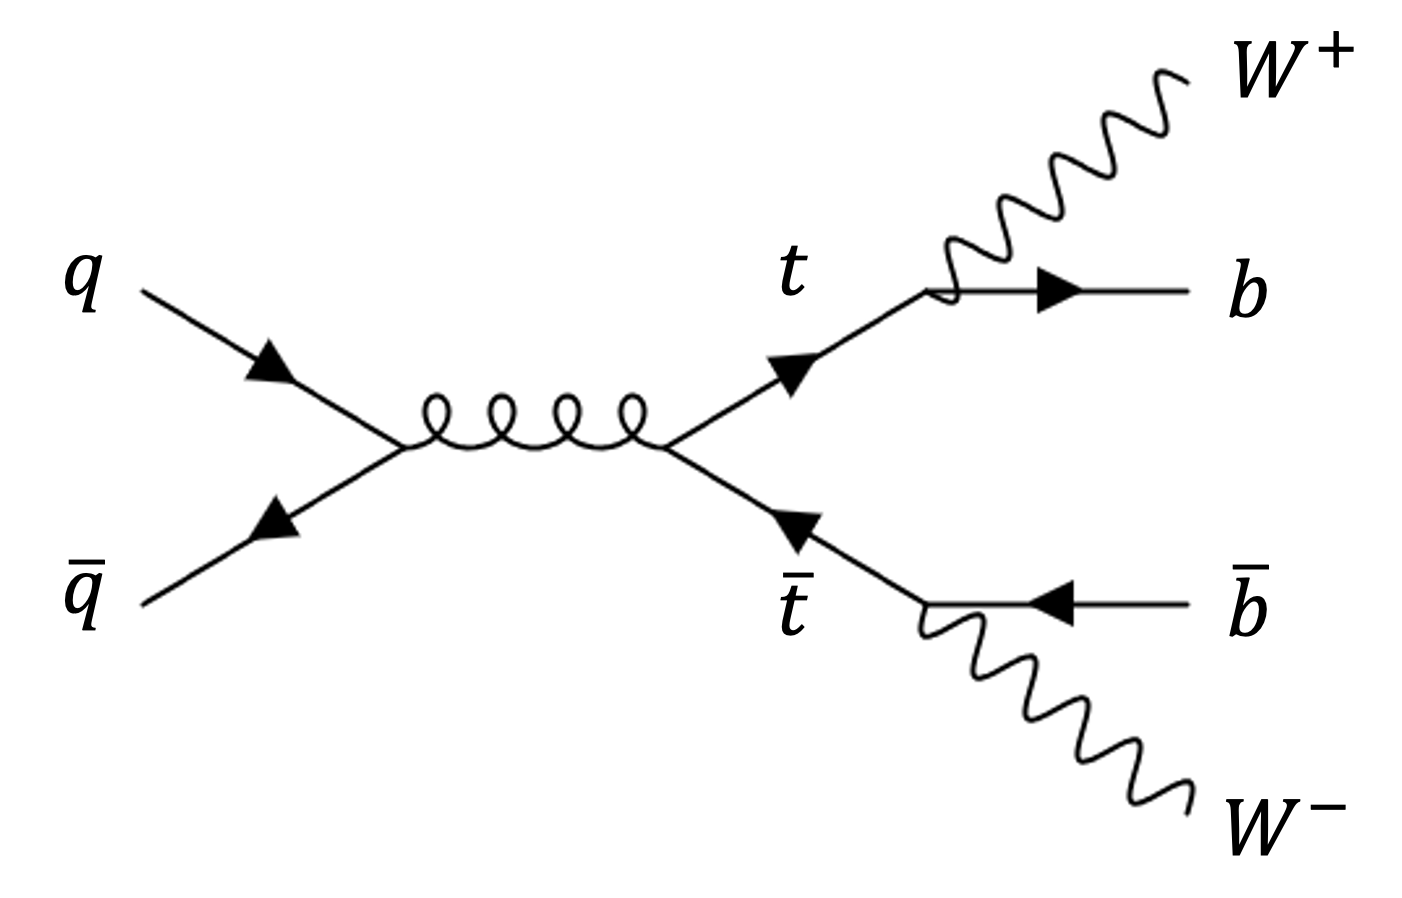
\includegraphics[width=0.5\textwidth]{Images/VH/Feynman/ttb.png}
  \caption{Feynman diagrams of the \ttb\ production and decay, where each $W$ can decay leptonically or hadronically.} 
  \label{fig:feynttb}
\end{figure}

\paragraph{Alternative samples} Several alternatives are simulated for modelling studies:
\begin{itemize}
  \item $PH7$: replacing \textsc{Pythia} by \textsc{Herwing} 7.0 with H7UE tune \cite{herwig7R} for parton shower, hadronisation, and \gls{ue}s while keeping the same nominal \textsc{Powheg} setup. This sample is used to systematically vary the parton shower model.
  \item $aMC$: based on \textsc{MadGraph5\_aMC\@NLO} \cite{madgraph} for NLO hard-scattering matrix element modelling with the nominal \textsc{Pythia} for \gls{ps}, hadronisation, and the \gls{ue} simulation. This samples is used to systematically vary the matrix element prediction.
  \item Weights variations tuning the initial and final state radiations (\gls{isr} and \gls{fsr}) contributions relative to the nominal setup. There are 4 such variations, based on the nominal \textsc{Powheg} + \textsc{Pythia} 8.230:
  \begin{itemize}
    \item 2 \gls{isr} variations named \textit{RadLow} and \textit{RadHigh}, where the $\mu_r$ and $\mu_f$ scales are doubled and halved\footnote{For \textit{RadHigh}, the \textit{hdamp} parameter is doubled from its nominal value of 1.5 $\times$ $m_{\text{top}}$.}.
    \item 2 \gls{fsr} variations, with an up (down) variation obtained by doubling (halving) the renormalisation scale $\mu_{r,\, FSR}$. % TODO Check these doubling and halving are still true, it's from Maria's thesis
  \end{itemize}
\end{itemize} 

\subsubsection{Single-top Production}
The so-called single-top process combines different minor channels, with the leading Feynman diagrams depicted in Figure~\ref{fig:feynstop}. The dominant contribution is the associated top-production $Wt$ channel, with the $t \rightarrow Wb$. Two other contributions are the $t$- and $s$-channel, with the former having a significantly increased cross-section over the later $s$-channel. These processes are simulated similarly to the \ttb, with the cross-sections calculated for a top-quark mass of $m_t = 172.5$ GeV at NLO in \gls{qcd} for the $s$- and $t$-channel \cite{ALIEV20111034, KANT201574} and with approximate NNLO accuracy from NNLL soft-gluon resummation for the fiducial $Wt$ production cross-section \cite{PhysRevD.82.054018, kidonakis2013quark}.
\begin{figure}[h!]
  \center
  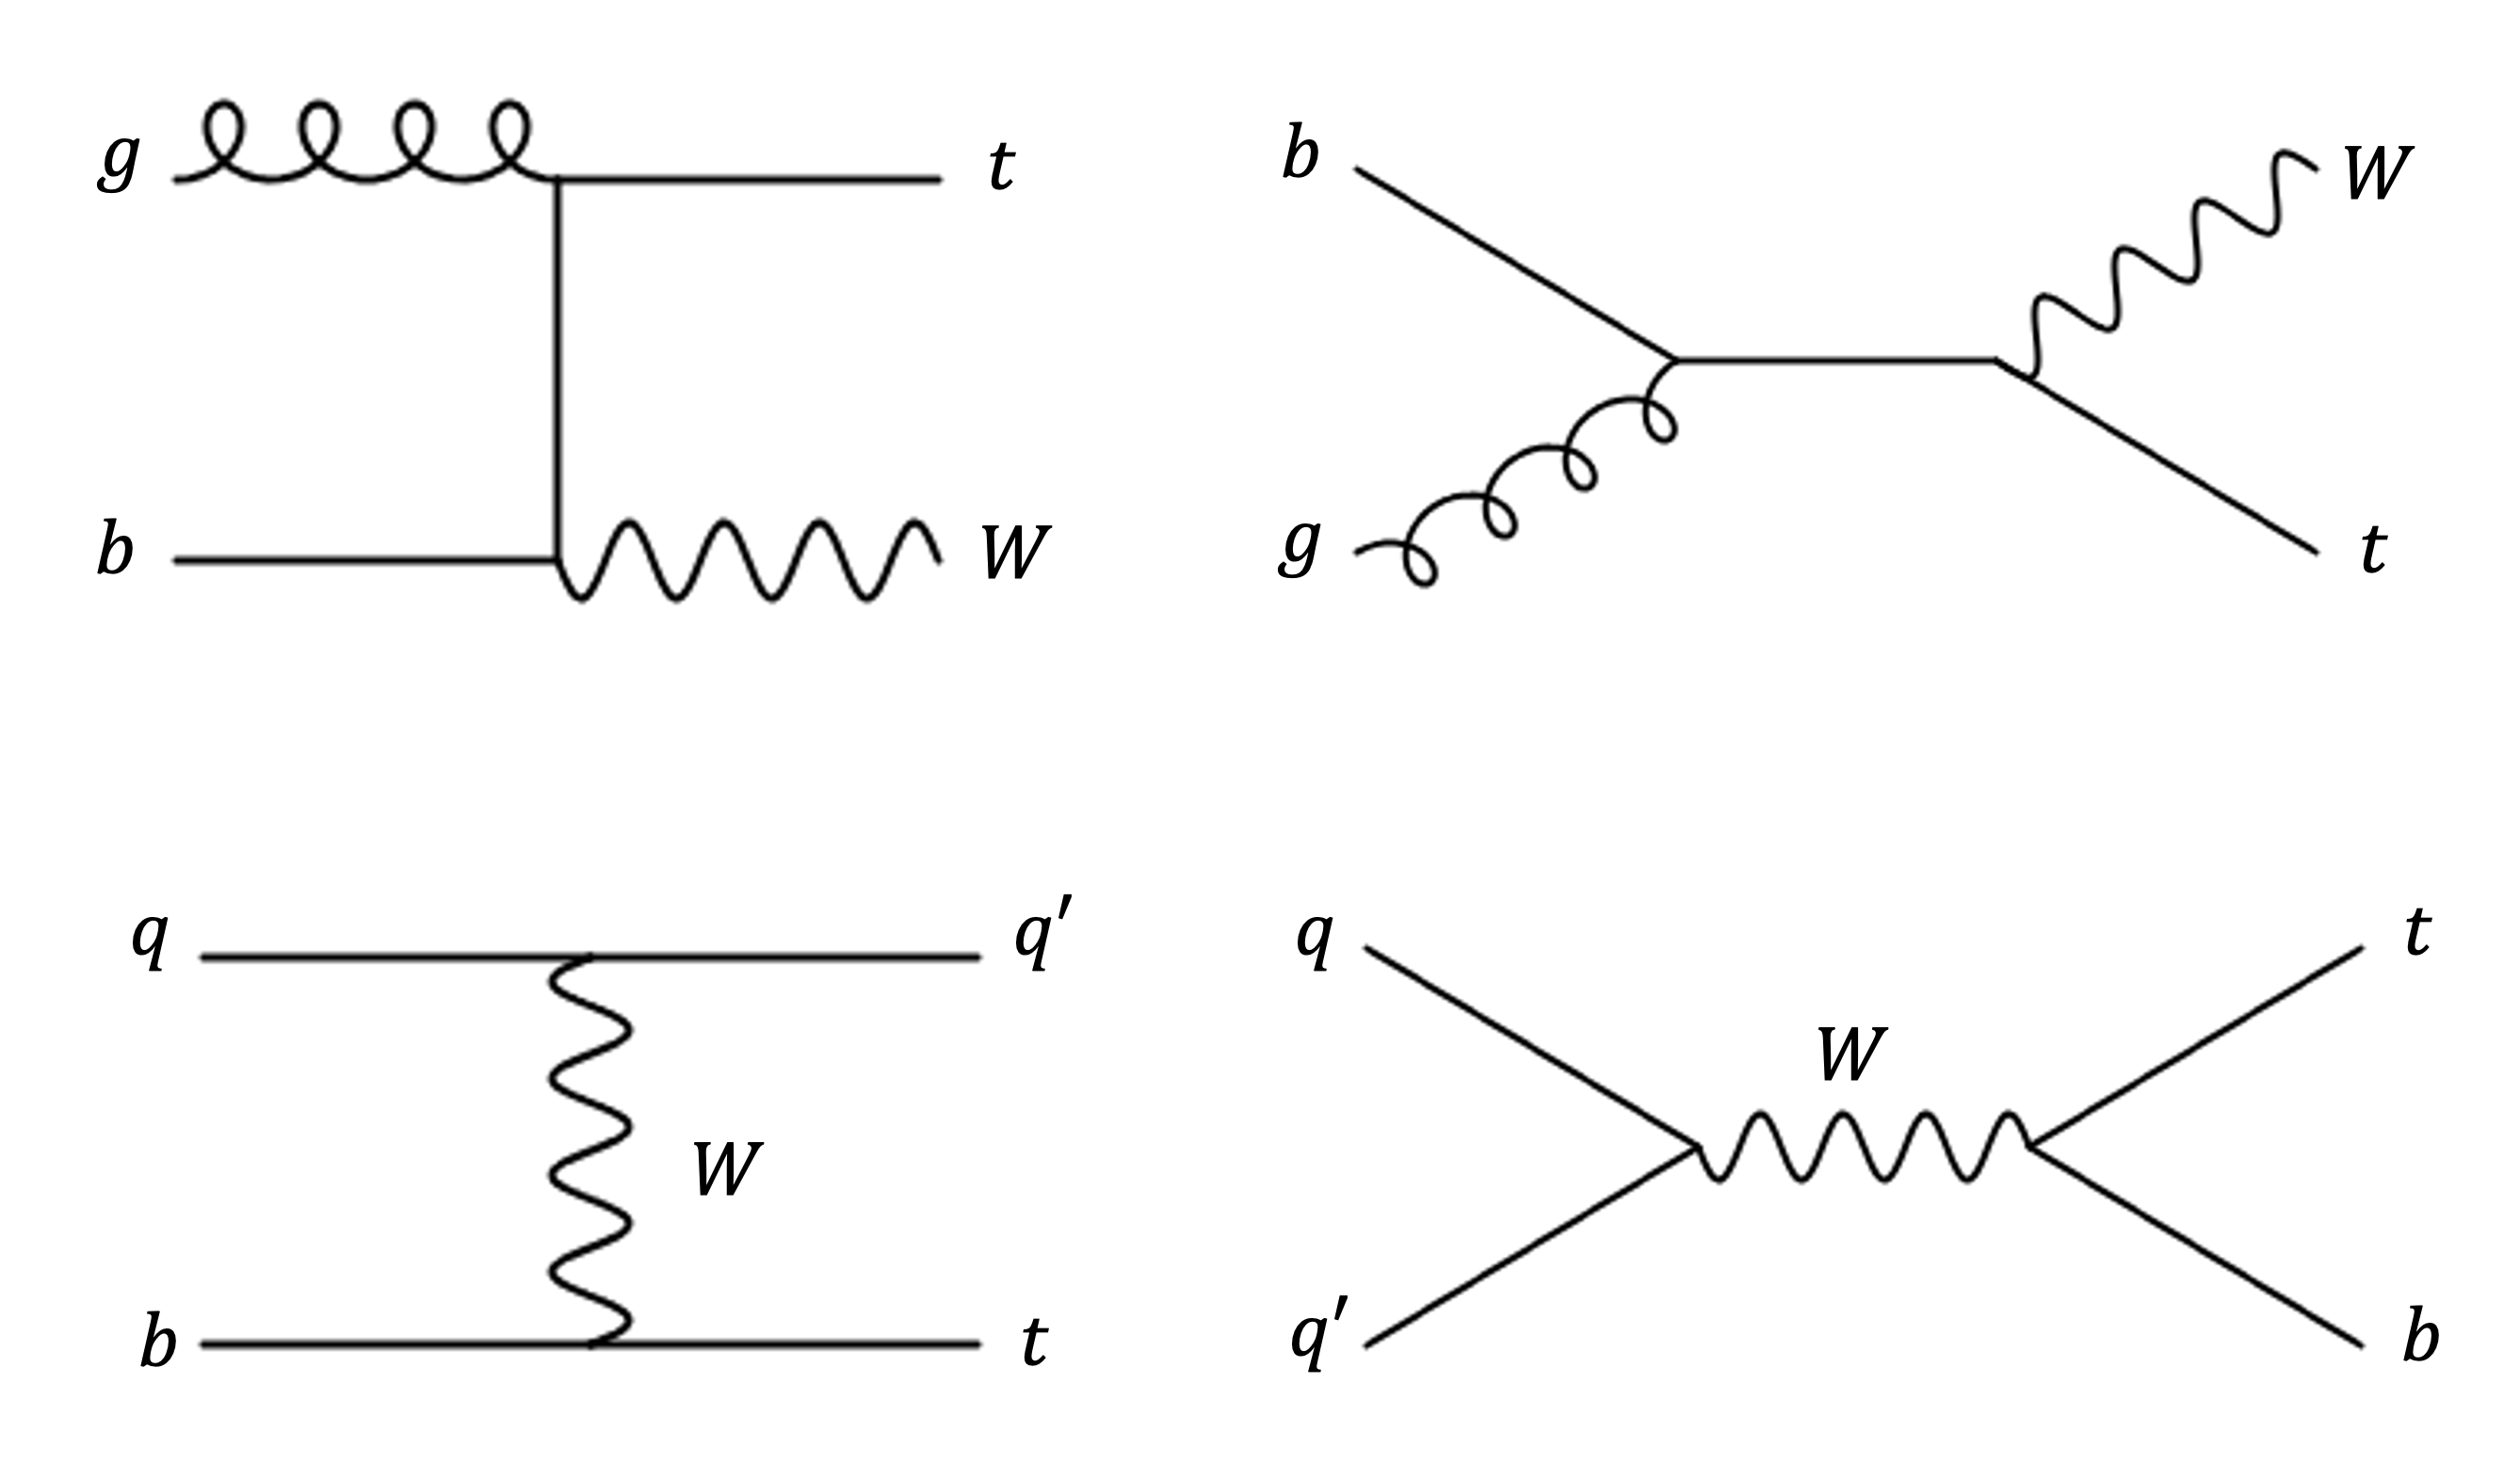
\includegraphics[width=0.7\textwidth]{Images/VH/Feynman/singletop.png}
  \caption{Feynman diagrams of the $Wt$-production (top) and the single top production (bottom) in the $t$-channel (left) and the $s$-channel (right).} 
  \label{fig:feynstop}
\end{figure}

The $Wt$ production channel has diagrams overlapping with the \ttb production at NLO in \gls{qcd}. In the analysis, a diagram sustraction (\textit{DS}) scheme is applied to remove the overlap with \ttb by locally cancelling the \ttb contribution in the NLO $Wt$ cross-section calculation \cite{StefanoFrixione_2008}. 

\paragraph{Alternative samples} Alternatives are used for the modelling of the single-top $Wt$- and $t$-channels\footnote{No alternatives are derived for the single-top $s$-channel due to its small contribution in the analysis.}:
\begin{itemize}
  \item The 6 alternative generators used for the alternatives of \ttb are also applied for the $Wt$- and $t$-channels.
  \item For $Wt$ only, a sample using an alternative overlap removal procedure is produced with the alternative diagram removal (\textit{DR}) scheme \cite{StefanoFrixione_2008} to systematically model the overlap with \ttb. This scheme removes the diagrams in the NLO $Wt$ amplitudes that are doubly-resonnant, when both $t$-quark on-shell. $DR$ was the default scheme in prior iterations of this analysis, but the $DS$ samples showed better agreement with data in the boosted regime and were therefore chosen as nominal.
\end{itemize}

\subsubsection{Di-boson Process}
The diboson processes $WW$, $WZ$, and $ZZ$ enter the analysis both as a background, with a hadronically decaying $V$ boson mistaken for the Higgs, and as a cross-check signal. Some leading $qq$-initated Feynman diagrams are depicted in Figure \ref{fig:feyndiV}, with gluon-initiated diagrams also possible via quark-loops. The $qq$-initiated di-boson are simulated similarly to the $V+$jets, using \textsc{Sherpa} 2.2.11 \cite{10.21468/SciPostPhys.7.3.034}. The $gg$-initiated are simulated with the older \textsc{Sherpa} 2.2.2 version. In both case, the cross-sections are computated at NLO precision, with the NNLO \gls{pdf}s based on NNPDF3.0nnlo \cite{PDFLHCrun2} for both the matrix element and parton shower.
\begin{figure}[h!]
  \center
  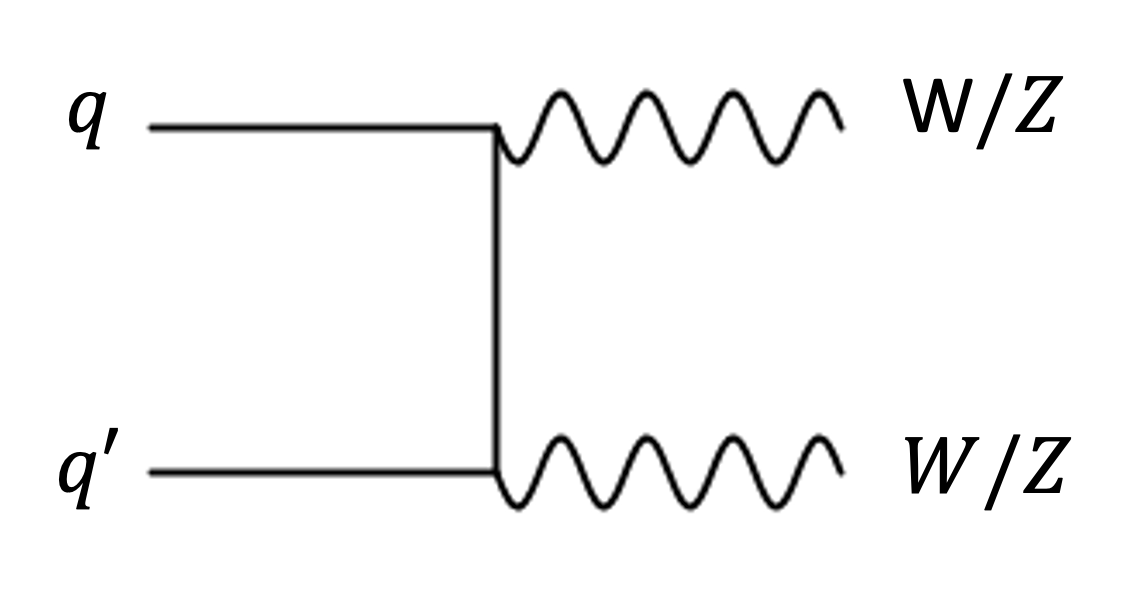
\includegraphics[width=0.32\textwidth]{Images/VH/Feynman/diboson.png}
  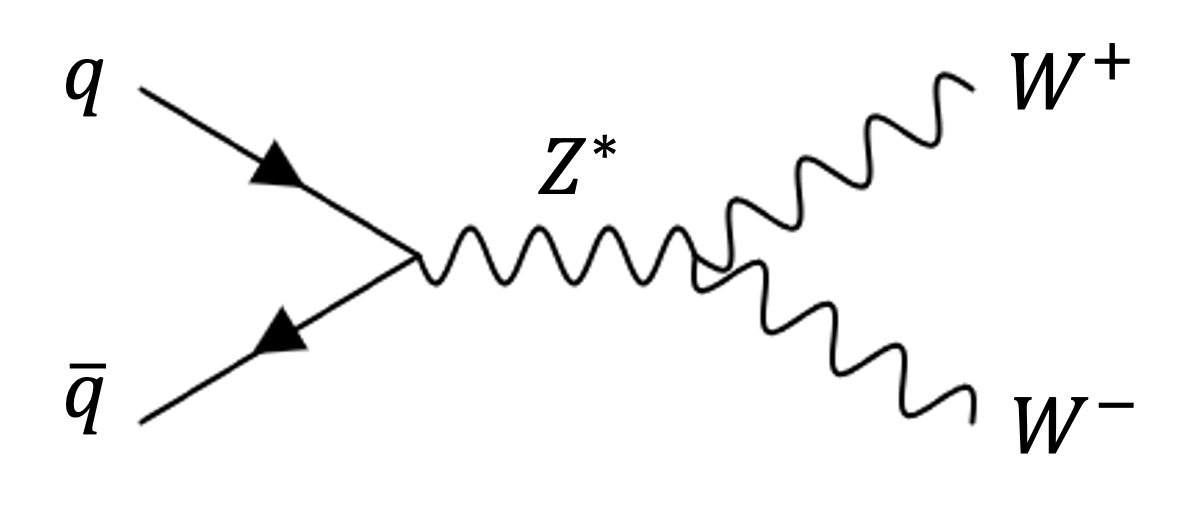
\includegraphics[width=0.32\textwidth]{Images/VH/Feynman/diW.png}
  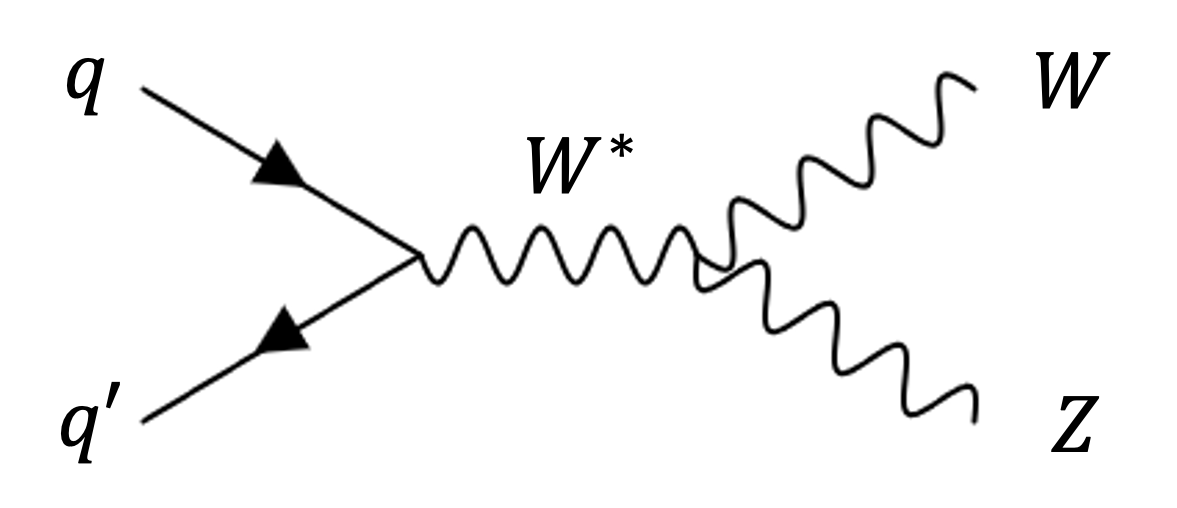
\includegraphics[width=0.32\textwidth]{Images/VH/Feynman/diWZ.png}
  \caption{Feynman diagrams of the di-boson production in the $t$- (left) and $s$-channel (centre \& right). The $t$-channel can lead to any combination of $W$ and $Z$ dependingon theinitial quark-pair.}
  \label{fig:feyndiV}
\end{figure}

\paragraph{Alternative samples:}
\begin{itemize}
  \item \textsc{Powheg} v2 interfaced with \textsc{Pythia} 8 for the \gls{ps} samples are produced to systematically assess \gls{me} and \gls{ps} variations. 
  \item \textsc{Sherpa} 2.2.1 samples are produces to systematically model the impact of the varying the fragmentation function.
\end{itemize}

\subsubsection{QCD Multi-jet}
This process is estimated from data instead of simulations because of the difficulty in generating a sufficient statistics samples due to the low selection efficiency, despite having a much larger production cross-section than the Higgs. \gls{qcd} multi-jet events can be selected when heavy flavour hadrons decay semi-leptonically or jets are mis-identified as leptons. Such leptons are normally not isolated, and only a small fraction passes the lepton requirements. The multi-jet is negligible in the 0-lepton and 2-lepton channels thanks to the strict selections available. In the 1-lepton resolved channel, the remaining contribution is assessed from data-driven templates. The residual multi-jet is mostly present at low \ptv values and is therefore ignored in the boosted regime. \\

%In the template method, the shape of the multi-jet is derived in a special control region \textit{mjCR} enriched in \gls{qcd} events, with the multi-jet normalisation factor free-floated in the signal region fit. Independent templates fits are performed for the electron and muon channels in the low and medium \ptv regions\footnot{Respectively $[75, 150]$ GeV, and $[150, 400]$ GeV.}, for 2- and 3-jet categories separately. The mjCR is obtained by inverting some the tight isolation cuts for the lepton and requiring only 1 $B$-tag to increase statistics. The distribution of $m_T^W$ in the mjCR is used in the fit as it gives the best discrimination between multi-jet and the other processes. Indeed, the main other backgrounds in the mjCRs are the $W+$jets and \ttb, which both have a characteristic peak close to the $W$-mass while the multi-jet as a smoothly falling distribution.

% TODO hard to fully describe the multi-jet.